
\section{Highlighters (settings)}
\index{secrets!colors preference}
\index{secrets!highlighters preference}

\texttt{Highlighters settings} is a window that allows you to customize the text you are working with in relation to appearance.
Usually, you will be working with \RR{}, R doc, R noweb, Tex or Text files.
The type of file is marked automatically at the left column of the window \texttt{Highlighters}.
Within the \texttt{Identifiers} section of the selected highlighter you may choose the foreground (FG)
color and the background color (BG) of each highlighter. Since the best configuration of BG is the same for every
identifier it is possible to set BG for all at once; use a dark color for BG.

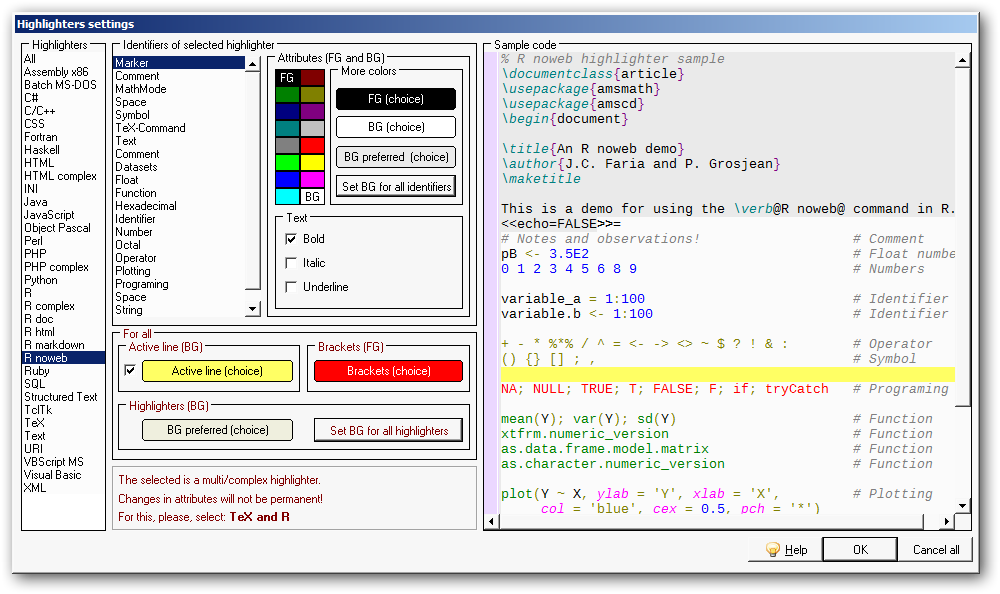
\includegraphics[scale=0.50]{./res/highlighter_settings.png}

The option \texttt{Options/Syntax(highlighter)} is used to set the highlighter of the type of file you would like,
provided it is not the same as the one you are currently working on.
